% !TEX root = main.tex
\chapter{Aerodynamic Effects on Vehicle Performance}
\label{chap:vehicleperformance}

  The first argument to the importance of aerodynamics is based on two facts: The fact that drag is negligible in regards to the Formula Student vehicle's top speed on straights, and the fact that aerodynamically increasing the vehicle's \emph{effective} mass due to downforce increases tyre grip, which in turn allows for higher cornering velocities.

  The second part of this chapter covers the importance of centering the effective mass increase due to aerodynamic devices close to the center of gravity -- otherwise handling characteristics becomes a function of velocity.

\section{Drag Effects on Straights}
\label{sec:topspeed}

  \begin{figure}
    \makebox[\textwidth][c]{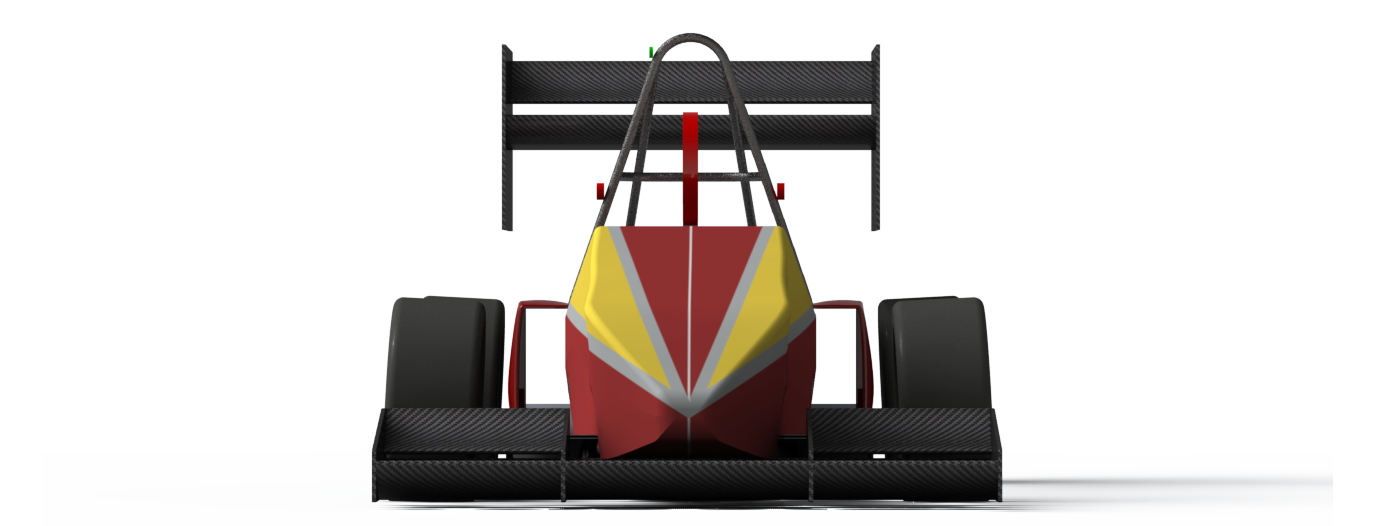
\includegraphics[width=2\textwidth]{frontalarea.png}}
    \caption{Frontal area of the car with a dummy wing inserted into the CAD model, in order to get an estimate of the drag coefficient $C_D$.}
    \label{fig:frontarea}
  \end{figure}

  First, let's explain what makes a car fast, and what parameters we can change to improve the speed of our car. The car's acceleration can be described by Newton's second law as:
  \begin{align}
    \sum F_x &= m a
    \intertext{Where the sum of forces working in the x-direction (the direction of travel) can be expressed as the force already pertained by the vehicle: The force the motor exerts is given by $F = \frac{P}{\dot{x}}$, where $P$ is the power of the car, minus the drag force:}
    F_D &= \frac{1}{2} C_D \rho \dot{x}^2 A\\
    F_\text{motor} &= m \ddot{x} = \frac{P}{\dot{x}}\\
    \sum F_x &= F_\text{motor} - F_D = \frac{P}{\dot{x}} - C_D \left(\frac{1}{2}  \rho \dot{x}^2 A \right) = 0
    \intertext{Where $C_D$ is the drag coefficient of the vehicle, $\rho$ is the density of the fluid it moves in and $A$ is frontal area of the vehicle. Solving for maximum speed, that is, when the two forces sum to zero:}
    F_\text{motor} &= F_D
    \intertext{As we were interested in the max speed of the car, let's solve for the velocity, giving:}
    \dot{x} &= \left( \frac{2 P}{C_D \left(\rho A \right)}\right)^{\frac{1}{3}}
  \end{align}
  This is assuming we're traveling at terminal velocity -- that is, the point where the $\text{Driving Force} = \text{Friction Force}$. The terminal velocity of the racer is then easily calculated, as the competition restricts the maximum amount of power to $\SI{80}{\kilo\watt}$, and the frontal area of the car is approximated from the CAD drawing seen in figure \ref{fig:frontarea}.

  \begin{align}
    \dot{x}_\text{max} &= \left(\frac{2\cdot \SI{80}{\kilo\watt}}{0.85\left(\SI{1.225}{\kilogram\per\cubic\metre}~ \SI{0.99 }{\square\metre}\right)}\right)^{\frac{1}{3}} = \SI{53.7}{\metre\per\second} = \SI{193.5}{\kilo\metre\per\hour}
    \intertext{however, given the ruleset a forecasted maximum of $\SI{110}{\kilo\metre\per\hour}$ allows a much larger drag coefficient $C_D$:}
    C_D &= \frac{2 P}{\dot{x}^3 \left(\rho A \right)}
    = \frac{2 \cdot \SI{80}{\kilo\watt}}{(\SI{110}{\kilo\metre\per\hour})^3 \left(\SI{1.225}{\kilogram\per\cubic\metre}~ \SI{0.99}{\square\metre} \right)} = 4.62
  \end{align}
  Thus, the car's top speed will only be limited by a drag factor $>4.62$, which is far above the drag introduced by the aerodynamic devices.

  From this derivation, it is clear that the car's abilities at maximum speeds far exceed the requirement of the track. Therefore, the next step is to improve cornering speeds which depend strongly on the tyre's grip on the surface of the road \cite{jkatz}.

  \section{Downforce Effects on Cornering}

    Shown before, drag does not limit the car's performance on straights. During cornering, drag is not an issue either, but the grip of the tyres limits the maximum velocity before the vehicle loses traction due to the centripetal force which is given by: \cite{taylor2005classical}
    \begin{align}
      F_\text{centripetal} &= \frac{m\dot{x}^2}{r}
      \intertext{where $r$ is the distance to the center of the cornering circle. The frictional force the car exerts due to downforce and tyre grip is given by:}
      F_\text{friction} &= \mu F_\text{normal} \label{eq:downforcetocorneringspeed}
      \intertext{where the normal force is given by both the weight and (negative) lift of the car, which serves as an effective mass increase:}
      F_L &= \frac{1}{2}C_L \rho  A \dot{x}^2\\
      F_\text{friction} &= \mu \left(mg + \frac{1}{2} C_L \rho  A \dot{x}^2 \right)
      \intertext{The vehicle will lose traction when the frictional force is less than the centripetal force.}
      \frac{m\dot{x}^2}{r} &> \mu \left(mg + \frac{1}{2} C_L \rho  A \dot{x}^2 \right)
      \intertext{Giving the maximum velocity for a given corner radius before the car skids out:}
      \Rightarrow \dot{x} &< \left(\frac{2\mu mg r}{m - \mu C_L \rho r  A}\right)^{\frac{1}{2}}
    \end{align}
    Again, the forecasted variation in radii of corners is prescribed by the rules to be between \SIrange{3}{50}{\metre}\cite{FSrules18}. Plotting this for various $C_L$ values between $1.5$ to $2.6$ \cite{CLvalues}, assuming $m=\SI{300}{\kilogram}$, $\mu = 1.5$ \cite{tyrefriction} and $A = \SI{0.99}{\square\metre}$ as previously used. The result can be seen in figure \ref{fig:cornerspeedvslift}.
    \begin{figure}
      \makebox[\textwidth][c]{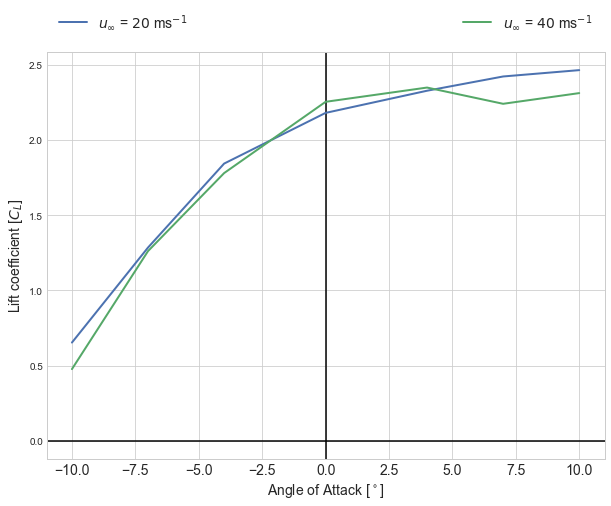
\includegraphics[width=1.2\textwidth]{turnspeedperCL2}}%
      \caption{Cornering speed as a function of turn radius for various lift coefficients.}
      \label{fig:cornerspeedvslift}
    \end{figure}

\section{Load Distribution}

  The scope of this thesis is not to incorporate a full aerodynamic package, but a quick overview of load distribution is essential to understanding the behaviour of the car.

  The effective mass added from negative lift depends on the lift coefficient. It is evident that different items on the car carry different lift coefficients, thus making the lifting forces over the cars length a function of relative speed. For the unexperienced driver, this is not easily managed as handling characteristics change with velocity. Therefore, it is desirable to have the aerodynamic center of pressure close to the car's center of gravity, in order to have similar handling at all velocities. While this is not handled in this thesis, it is ideal for future iterations and essential for a full aerodynamical package.

%Check https://uta-ir.tdl.org/uta-ir/bitstream/handle/10106/24176/Merkel_uta_2502M_%2012503.pdf?sequence=1
